\documentclass[tikz,border=3pt]{standalone}
\usepackage{newtxtext,newtxmath}
\usetikzlibrary{arrows.meta,positioning}
\definecolor{paperblue}{HTML}{2F6DB0}
\definecolor{paperred}{HTML}{C83E4D}
\definecolor{papergold}{HTML}{E3A008}
\definecolor{papergreen}{HTML}{2E8B57}
\begin{document}
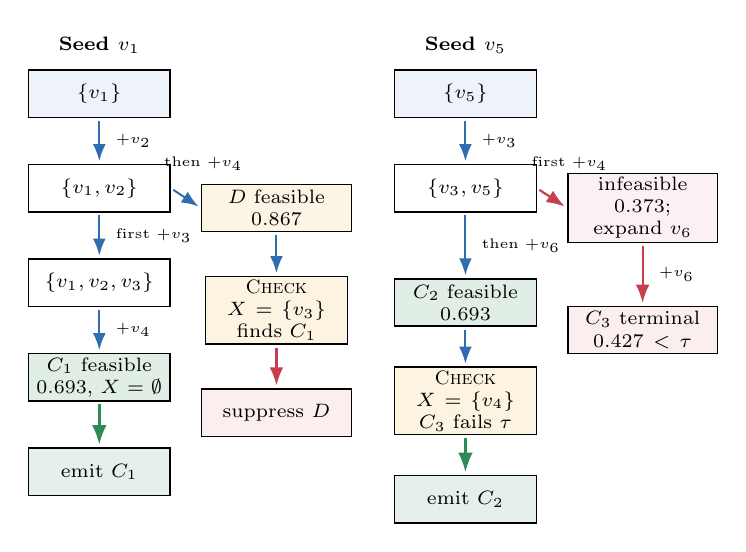
\begin{tikzpicture}[
  font=\scriptsize,
  >=Latex,
  state/.style={draw=black, line width=0.55pt,
    minimum width=18mm, minimum height=6.0mm, text width=17mm, align=center,
    fill=white, inner xsep=0.45mm, inner ysep=0.45mm},
  side/.style={state, minimum width=19mm, text width=18mm},
  flow/.style={->, line width=0.7pt, draw=paperblue, shorten <=1pt, shorten >=1pt},
  fail/.style={->, line width=0.8pt, draw=paperred, shorten <=1pt, shorten >=1pt},
  check/.style={state, fill=papergold!12},
  label/.style={font=\scriptsize\bfseries, text=black}
]
% A feasible candidate may still be suppressed by the exclusion-set check.
\node[label] at (-2.75,0.62) {Seed $v_1$};
\node[state, fill=paperblue!8] (v1) at (-2.75,0) {$\{v_1\}$};
\node[state] (v12) at (-2.75,-1.20) {$\{v_1,v_2\}$};
\node[state] (v123) at (-2.75,-2.40) {$\{v_1,v_2,v_3\}$};
\node[state, fill=papergreen!15] (c1) at (-2.75,-3.60)
  {$C_1$ feasible\\$0.693$, $X=\emptyset$};
\node[state, fill=papergreen!13] (emit1) at (-2.75,-4.80) {emit $C_1$};
\draw[flow] (v1) -- node[midway,right=0.8mm,font=\tiny] {$+v_2$} (v12);
\draw[flow] (v12) -- node[midway,right=0.8mm,font=\tiny] {first $+v_3$} (v123);
\draw[flow] (v123) -- node[midway,right=0.8mm,font=\tiny] {$+v_4$} (c1);
\draw[->, draw=papergreen, line width=0.9pt, shorten <=1pt, shorten >=1pt] (c1) -- (emit1);

\node[side, fill=papergold!10] (d124) at (-0.50,-1.45)
  {$D$ feasible\\$0.867$};
\node[side, check] (check1) at (-0.50,-2.75)
  {\textsc{Check} $X=\{v_3\}$\\finds $C_1$};
\node[side, fill=paperred!9] (drop1) at (-0.50,-4.05) {suppress $D$};
\draw[flow] (v12.east) -- node[midway,above=2.2mm,xshift=2.2mm,font=\tiny] {then $+v_4$} (d124.west);
\draw[flow] (d124) -- (check1);
\draw[fail] (check1) -- (drop1);

% An infeasible intermediate is expanded while it still has a candidate child.
\node[label] at (1.90,0.62) {Seed $v_5$};
\node[state, fill=paperblue!8] (v5) at (1.90,0) {$\{v_5\}$};
\node[state] (v35) at (1.90,-1.20) {$\{v_3,v_5\}$};
\node[state, fill=papergreen!15] (c2) at (1.90,-2.65)
  {$C_2$ feasible\\$0.693$};
\node[check] (check2) at (1.90,-3.90)
  {\textsc{Check} $X=\{v_4\}$\\$C_3$ fails $\tau$};
\node[state, fill=papergreen!13] (emit2) at (1.90,-5.15) {emit $C_2$};
\draw[flow] (v5) -- node[midway,right=0.8mm,font=\tiny] {$+v_3$} (v35);
\draw[flow] (v35) -- node[midway,right=0.8mm,font=\tiny] {then $+v_6$} (c2);
\draw[flow] (c2) -- (check2);
\draw[->, draw=papergreen, line width=0.9pt, shorten <=1pt, shorten >=1pt] (check2) -- (emit2);

\node[side, fill=paperred!7] (f345) at (4.15,-1.45)
  {infeasible\\$0.373$; expand $v_6$};
\node[side, fill=paperred!9] (c3) at (4.15,-3.00)
  {$C_3$ terminal\\$0.427<\tau$};
\draw[fail] (v35.east) -- node[midway,above=2.2mm,xshift=2.2mm,font=\tiny] {first $+v_4$} (f345.west);
\draw[fail] (f345) -- node[midway,right=0.8mm,font=\tiny] {$+v_6$} (c3);
\end{tikzpicture}
\end{document}
